\chapter{Results}

\section{Description}
In this section, we go over the performance of the system's communication reliability and the cost of the system.

\section{Communication Reliability}
An area of concern with the wireless communication of the system involved interference between the 802.15.4 network and 802.11 Wi-Fi. Since both protocols use the same 2.4 GHz frequency, it's possible for packets to be lost due to channel interference. Figure \ref{fig:802154} shows the frequency coverage of each Wi-Fi and 802.15.4 channel. In order to maximize the reliability of our system, we use 802.15.4 channel 26 so that there is no overlap with any common Wi-Fi network. Most Wi-Fi devices go as high as channel 11, which would not interfere with any communication happening on 802.15.4 channel 26. Although dropped packets were rarely encountered in the early stages of testing, switching to channel 26 completely eliminated all packet loss in our test environment.

\begin{figure}[h]
  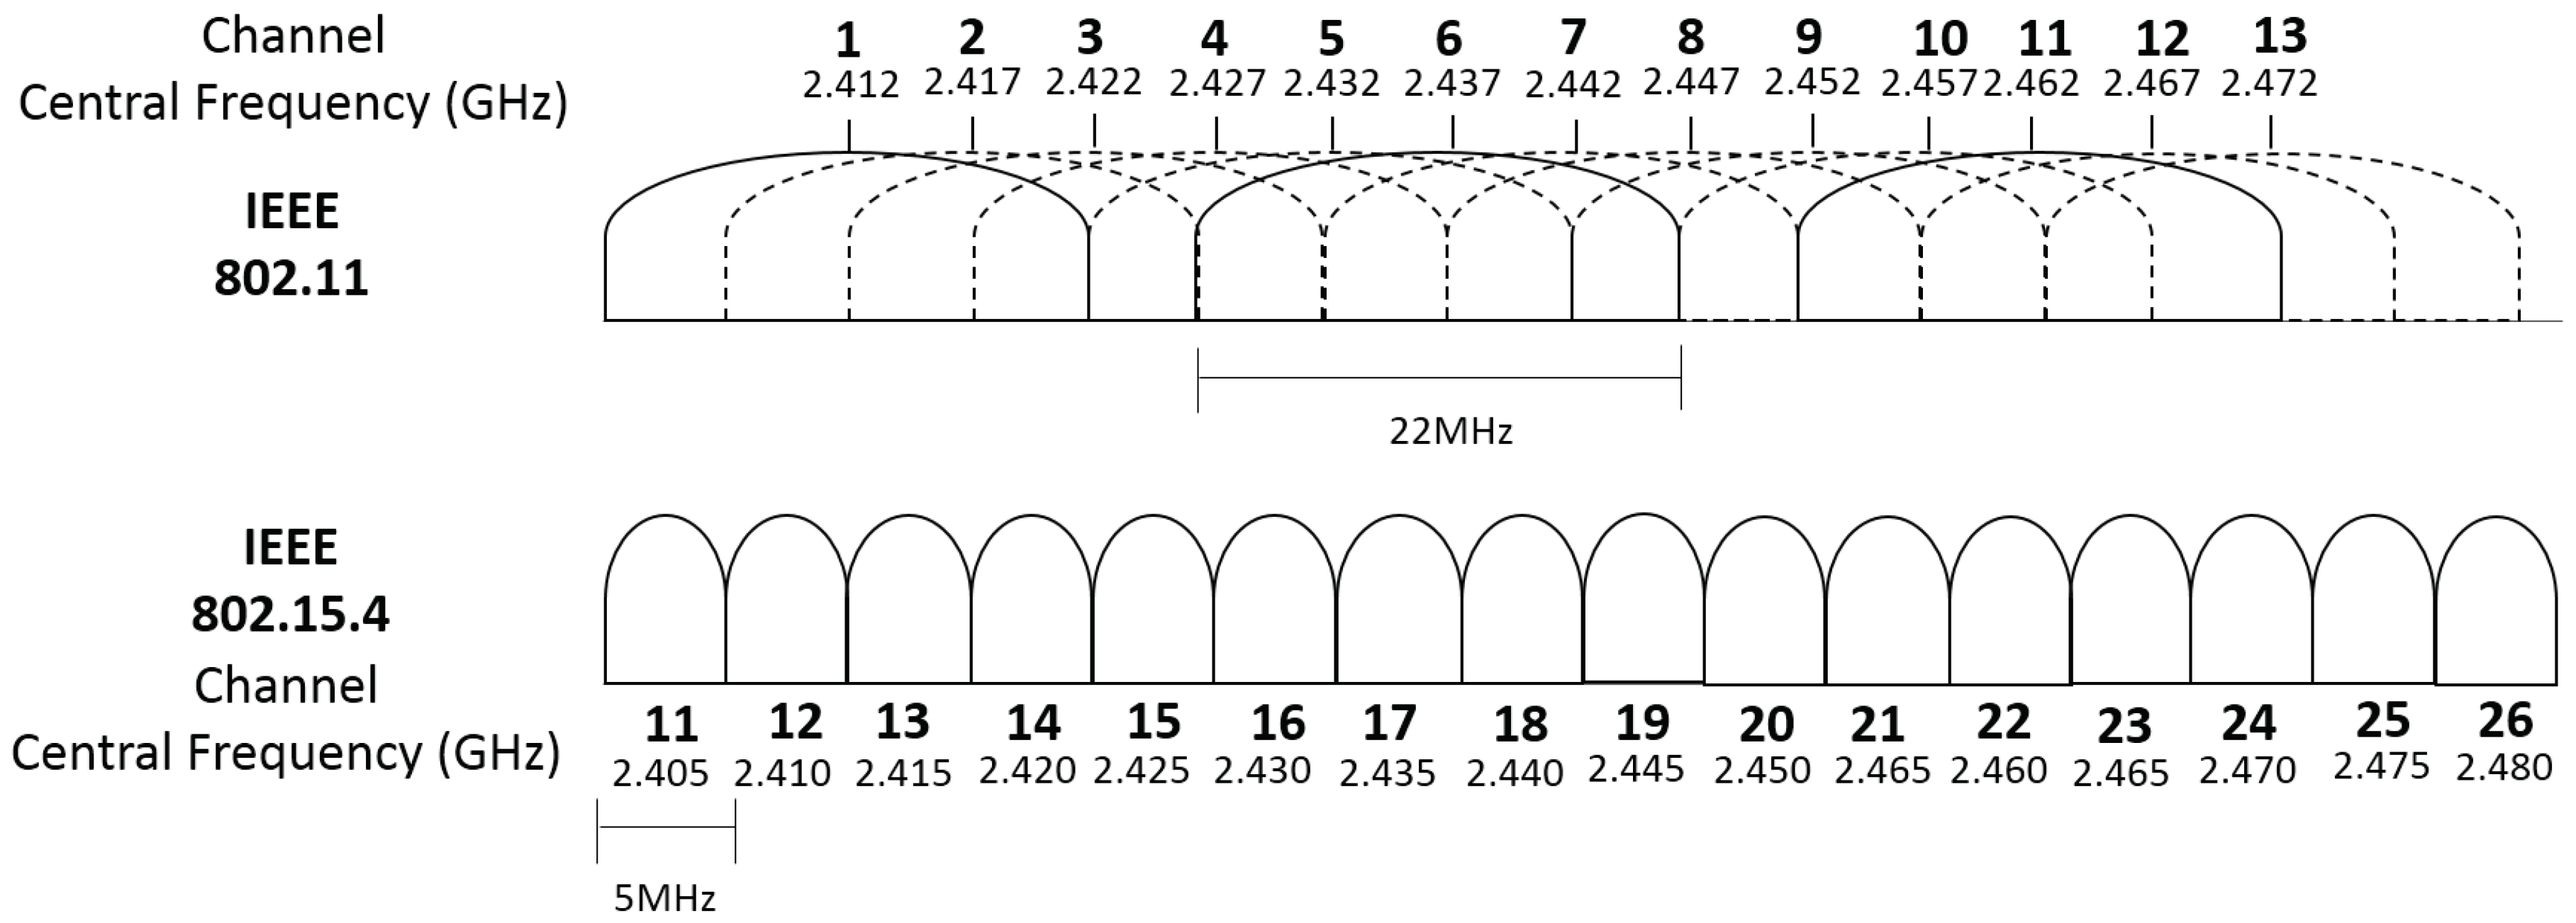
\includegraphics[width=0.8\textwidth]{802154.png}
  \centering
  \caption{IEEE 802.11 and 802.15.4 Channel Comparison \cite{pdf:802.15.4}}
  \label{fig:802154}
\end{figure}

\section{Cost}
One main goal of this project was to minimize the cost of an open, scalable system. In considering the costs of solely our system (the doorbell and gateway), we find the cost to be reasonable. A Raspberry Pi Zero W costs \$15. If a user were  to decide not to use the W variant and connect the Raspberry Pi Zero directly to the router through Ethernet, it would cost \$5 - \$10. In our implementation we did use Arduino Uno but an implementation could use the smaller and low power alternative, Arduino Nano which costs \$5 - \$10. Unfortunately, the expensive module in this design was the XBee module. The cost is around \$20 and we need two. The final cost is about \$50 - \$75. Of course, the resident would also have to purchase an IoT device that can send notifications. A possible affordable option would be a smart plug, which can effectively make any device a smart device. Cheapest options are around \$10. At the cheapest and most expensive options, the cost is at least below \$100. By some metrics, that may still be too expensive for individuals. Hopefully, as IoT starts to grow, we start to see small computers like Raspberry Pi and Arduino that implement 802.15.4 directly into the board.